\documentclass{article}
\usepackage[utf8]{inputenc}
\usepackage[portuguese]{babel}
\usepackage{csquotes}
\usepackage{graphicx}
\usepackage{adjustbox}
\usepackage{lipsum}
\usepackage[backend=biber,autolang=other,
  bibencoding=utf8,style=alphabetic,
  ibidtracker=true]{biblatex}
\addbibresource{polo-natural.bib}

\title{Franscisco d'Holanda e o Tirar Pelo Natural} \date{2 de
  Julho de 2015} \author{João Távora \\Faculdade de Belas Artes da
  Universidade de Lisboa}

\begin{document}

\maketitle

\section{Sinopse}

``Do Tirar Polo Natural'' é um pequeno tratado sobre retrato de
Francisco d'Holanda (1517 – 1585), arquitecto, ilustrador, humanista,
ensaísta e figura chave da Renascença Portuguesa. No diálogo conversam
Fernando e Braz Pereira, sendo o primeiro o próprio Francisco
d'Holanda e o segundo um amigo do autor residente no Porto. O presente
trabalho analisa os indícios bibliográficos e as contribuições
originais deste tratado, enquadrando-a na restante obra do autor.

\section{Palavras-chave}

Francisco d'Holanda, Desenho, Retrato

\section{Introdução}

``Do Tirar Polo Natural'' é um pequeno tratado em forma de diálogo que
surge na sequência de duas obras anteriores, ``Da Pintura Antiga'' e
``Diálogo em Roma''. O tema é a pintura ou o desenho de retrato ao
vivo. Segundo algumas fontes, trata-se do primeiro tratado da história
de arte sobre a este tema em
específico.\cite[p.11]{raphael}\cite{campbell} \footnote{Francisco da
  Holanda termina a obra em 1549 em Santarém. O original manuscrito
  encontra-se perdido, sabendo-se apenas que em 1790 estava em
  Espanha, nas mãos de D. José Calderón, que o emprestou a Diogo de
  Carvalho e Sampaio, diplomata em Madrid, que por sua vez o emprestou
  a Monsenhor Gordo para que dele se pudesse fazer uma cópia. É dessa
  cópia que Joaquim de Vasconcelos extraiu o texto que publicou em
  1892, e sobre o qual a edição consultada de José da Felicidade
  Alves\cite{holanda} se baseia. Existe uma tradução anterior para o
  espanhol, feita por Manuel Denis, contemporâneo de F. d'H., de
  1563. Esta inclui-se num Códice de obras de F. d'H. e que, seguindo
  um percurso diferente, se encontra hoje na Academia de São Fernando
  em Espanha. À cópia de Monsenhor Gordo, bem como à tradução
  espanhola, faltam alguns desenhos ilustrativos do próprio F. d'H aos
  quais é feita referência no texto e que se terão perdido com o
  manuscrito original.}

A obra estrutura-se num prólogo e 11 pequenos capítulos. No prólogo
explicam-se as circunstâncias da elaboração da obra, uma viagem a
Santiago de Compostela, da qual se proporciona um encontro com Braz
Pereira, amigo de infância de F. d'H. e interlocutor frequente deste
autor em matérias de arte.

Os dois primeiros capítulos introduzem o conteúdo teórico e delineiam
do posicionamento ideológico da obra, afirmando as ideias de perfeição
divina e génio do autor.

Os capítulos seguintes contêm um princípios pedagógicos sobre desenho
de retrato ao vivo, agrupados pelas partes do rosto que F. d'H. deseja
focar em cada capítulo. O conjunto destes preceitos visam mais o
desenvolvimento de uma maneira particular de artista do que um estudo
aprofundado sobre retrato. No último capítulo sintetiza-se do conteúdo
educativo e fazem-se referências a Miguel Ângelo e a Alberti. Em
apêndice, encontra-se ainda uma pequena nota de finalização
(``Acabei-o'') e a transcrição, em latim, de uma carta de Leão X a Rafael de
Orbino em latim.

O presente trabalho enquadrar este tratado na restante obra de
Francisco d'Holanda, focando, em sequência, os aspectos
auto-biográficos, ideológicos e artístcos nele contidos. No final
sintetizam-se as conclusões retiradas.

\section{Aspectos biográficos}

Segundo o Francisco d'Holanda, foi numa particular etapa de uma viagem
do autor a Santiago de Compostela com o infante D. Luís que se
proporcionou uma paragem no Porto, onde o tomou por hóspede Braz
Pereira, filho de Fernando Brandão, antigo fidalgo ao serviço do
infante D. Fernando. F. d'H. explica como terá sido durante a infância
criado com Braz Pereira, e que lhe foi fácil aceitar a oferta de
hospitalidade.

O autor declara que a estada em casa de Braz Pereira é frequente, e
como lhes é costume discutir pintura e arquitectura nessas ocasiões,
``gastando nisso parte das noites'', mas insiste em clarificar que
nesta ocasião é uma encomenda do próprio infante D. Luís, de quem se
aparta em Amarante, de que através de uns intermediários, se
entregassem a Braz Pereira umas cabeças de gesso antigas existentes em
Santo Tirso e provindas de Roma, para que finalmente pudessem estas
ser expedidas para Lisboa por via marítima.

E é nessa estadia de ``oito dias, de vida boa'' em casa de Braz
Pereira, que se produz segundo F. d'H. o desejo de registar as
observações que ali se produziam sobre pintura ao natural. E
declarando o autor que ``será melhor ouvir o que cada um dizia nesta
prática que perder-se mais o tempo''\cite[p12]{holanda}, justifica
desta forma a escolha da forma do diálogo para o livro.

O prólogo d'``[o] Tirar Pelo Natural'' é fértil em indícios
biográficos sobre Francisco de Holanda.

Nas notas à edição consultada \cite{holanda}, José da Felicidade Alves
estuda em particular a referência à povoação de Amarante e ao culto de
São Gonçalo, frade dominicano do século XIII, a quem é atribuída,
entre outras obras, uma ponte sobre o rio Tâmega, edificada para
livrar o povo dos perigos do vau. É em 1540 que começariam as obras da
igreja que abrigaria o sepulcro do santo. Segundo J. F. Alves é esta
construção em curso que teriam levado F. d'H. a visitar a povoação em
1548, na qualidade de arquitecto e não apenas de peregrino religioso.

A relevância à referência às ``cabeças de gesso'' de que fala
F. d'H. é também explorada por J. F. Alves. D. João III travava
durante o seu reinado uma luta contra D. Miguel da Silva, bispo de
Viseu ordenado cardeal em 1539 pelo papa Paulo III, e por essa altura
relocado em Roma. O património desse cardeal em Portugal estaria a
cargo de um outro cardeal Farnésio, em Santo Tirso. A incumbência de
F. d'H. seria tentar recuperar parte do espólio de arte de D. Miguel
da Silva.

Existe ainda uma referência à cidade do Porto como ``cidade
estrangeira em Portugal''. J. F. Alves revela-se ignorante do
significado desta sentença, enquanto Teresa Lousa\cite{teresa-desenho}
especula:

\begin{quote}
 O Porto seria uma cidade que se afigurava estranha aos olhos de um
 classicista. É uma cidade estrangeira porque é uma cidade
 gótica. Para o gosto humanista o gótico é o que está fora de moda e é
 sinal de mau gosto.  Para Holanda só o Antigo é digno de admiração e
 veneração.
\end{quote}

Por fim, F. d'H. refere uma obra anterior sobre pintura, ``um volume
em dois livros'', que é naturalmente o seu ``Da Pintura Antiga'',
terminado no ano anterior de 1548.

\section{Os mestres singulares}

Nos primeiro capítulos, Francisco d'Holanda consegue, em poucas
páginas, coser um fio condutor idelógico que liga a antiguidade
clássica à época presente e à sua própria pessoa.

Submetendo todo o relato à autoridade de Deus, como é naturalmente
obrigatório, F. d'H. narra a forma como Alexandre o Magno terá pedido
ao pintor Apeles que lhe pintasse o retrato de uma donzela
amada. Apeles ter-se-á apaixonado ele próprio por esta donzela, o
assim Alexandre ao pintor ``fez dela dom''\cite[p.13]{holanda}.

Exalta-se deste modo a pintura, e em particular a pintura ao natural,
como ``a coisa mais digníssima desta mundo e o tirar ao natural aquilo
que só Deus [...] sabe''. Ao que acrescenta:\cite[p.13]{holanda}

\begin{quote}
   Querê-lo um homem de terra imitar deve ser coisa mui grande e a
   maior que os homens podem fazer; ao menos eu (de o não saber fazer)
   por a maior a estimo; outros tê-lo-ão por menos.
\end{quote}

Neste parágrafo em que se deriva a ideia de perfeição da ideia de
divindade, F. d'H. remete-se à modéstia, e acrescenta à frente que a
``graça da perfeição'' é ``concedida a mui poucos dos
mortais''\cite[p.14]{holanda}.

F. d'H. afirma que só alguns merecem ser ``ao natural terladados'',
naturalmente os príncipes ou pessoas dignas. Esses não ``se devem fiar
senão de um eminente e singular desenhador''. Desta forma explica que,
tal como qualquer grande rei da antiguidade, o ``benigníssimo e
católico rei nosso senhor, que por resplendor de suas virtudes e
singular liberalidade merece mui justamente ficar em
memória''\cite[p.15]{holanda}. Referindo-se naturalmente a D. João
III, sugere que é o pintor que tem a responsabilidade de reconhecer e
preservar a memória dos grandes reis cuja relevança apenas mais tarde
será plenamente reconhecida\cite[p.15]{holanda}:

\begin{quote}
  [..] porque para falar dele como ele merece e eu entendo, não é tempo.
\end{quote}

Um pouco à frente, declara que quando nasce algum ``príncipe famoso'', logo com
ele nasce um ``escritor que o celebr[a] e [um] eminente pintor que o
mand[a] por tudo o mundo ao natural''.

Não é difícil perceber que, como observa José da Felicidade Alves nas
notas\cite[p.47]{holanda}, F. d'H. está aqui a fazer o seu próprio
elogio, algo que é completamente confirmado um capítulo mais tarde
quando o autor declara ter retratado D. João III ao natural.

É ainda neste capítulo que a estrutura de diálogo mais se assemelha ao
diálogo platónico original, sendo as perguntas de Braz Pereira
meramente figuras de pontuação e retórica para apoiar o discurso de
F. d'H.É. É também aqui que a mensagem ideológica e neo-platónica da
obra é mais evidente, ainda que não tão maturado como em obras
posteriores: o artista genial é ``agraciado'' por Deus com um ``saber
fazer'' que se aproxima do Dele\cite[p.14]{holanda}. Não figura aqui
ainda o conceito de ``desenho como ideia'' tão desenvolvido como n'``A
Ciência do Desenho''\cite{holanda-desenho}, no entanto não se anda
longe dele.

\section{A relação com o modelo}

Nos capítulos 3 a 10 trata-se, em variados graus de pormenor, a
abordagem correcta às várias partes da fisionomia no retrato,
começando-se pelos olhos e acabando no vestido. São desenvolvidos os
``primores de artista'', como saber fazer os olhos, as sobrancelhas, o
perfil gracioso do nariz, a intensidade da cor a dar na boca, bem como
os realces a branco.

No entanto, é só no capítulo 11º, ``Finais avisos no tirar ao
natural'', que surgem as indicações mais interessantes e se
desenvolvem as ideias mais originais de todo o tratado. Com efeito,
apesar de apelar durante os capítulos anteriores a um um sentido de
observação o mais agudo possível e que o pintor ``imite a verdade do
que tira''\cite[p.31]{holanda}, lê-se neste capítulo a seguinte
troca\cite[p.39]{holanda}:

\begin{quote}
  [...] e se for pessoa de pouca idade, pareça ainda de menos idade:
  \emph{Braz Pereira -}  E se for de muita idade?
  \emph{Fernando -}  Pareça ainda, se quiserdes, de menos idade.
  \emph{Braz Pereira -}  E se for pessoa fremosa?
  \emph{Fernando -}  Pareça ainda mais fremosa.
\end{quote}

Já no capítulo ``Como nenhuma obra obra perfeita deve ser vista antes
de ser acabada'', F. d'H. relata um episódio vivido por seu pai
António d'Holanda aquando de um retrato ao natural de ``César, o
imperador''\footnote{O Autor refere-se, naturalmente, a Carlos V,
  imperador do Sacro Império Romano-germânico.}\cite[p.17]{holanda}: O
rei ter-se-á ele próprio oferecido para ajudar o artista a ajustar o
seu cavalete, evitando assim que alguém entrasse para perturbar o
artista. Mais à frente, F. d'H. revela como teve que pedir a D. João
III que ``mande ao conde [da Castanheira] que se afaste para uma
parte, porque, estando ele diante, não [pode F. d'H.] fazer o que
deseja quietamente, nem o que pertence à perfeição da obra''. A
propósito dos efeitos nefastos dos ``indiscretos'', F. d'H. escreve
ainda\cite[p.18]{holanda}:

\begin{quote}
  Quero-vos ainda dizer mais: que se pudera ser estar [sic] o mesmo
  desenhador só, sem ninguém, e ter na fantasia e memória a pessoa que
  há-de pôr em obra e pintar, crêde que muito melhor seria que tê-la
  diante dos olhos visíveis se a visse com os invisíveis, quanto mais
  estar contentando a quantos indiscretos há numa corte e tê-los todos
  presentes, porque ao menos não lhe acontecesse querer pintar ao
  senhor diante dos seus criados, não os pintasse a eles todos no
  rosto dele.
\end{quote}

A interpretação da profundeza psicológica do retrato e das
interferências dos ``indiscretos'' na liberdade do artista só é tão
bem conseguida como neste texto, num desenho de um contemporâneo
holandês de F. d'H., Pieter Brueghel (1525-1569) \ref{fig:1}, sendo
claríssimo de observar nesse desenho exactamente a mesma tensão de que
fala Holanda.

\begin{figure}
\centering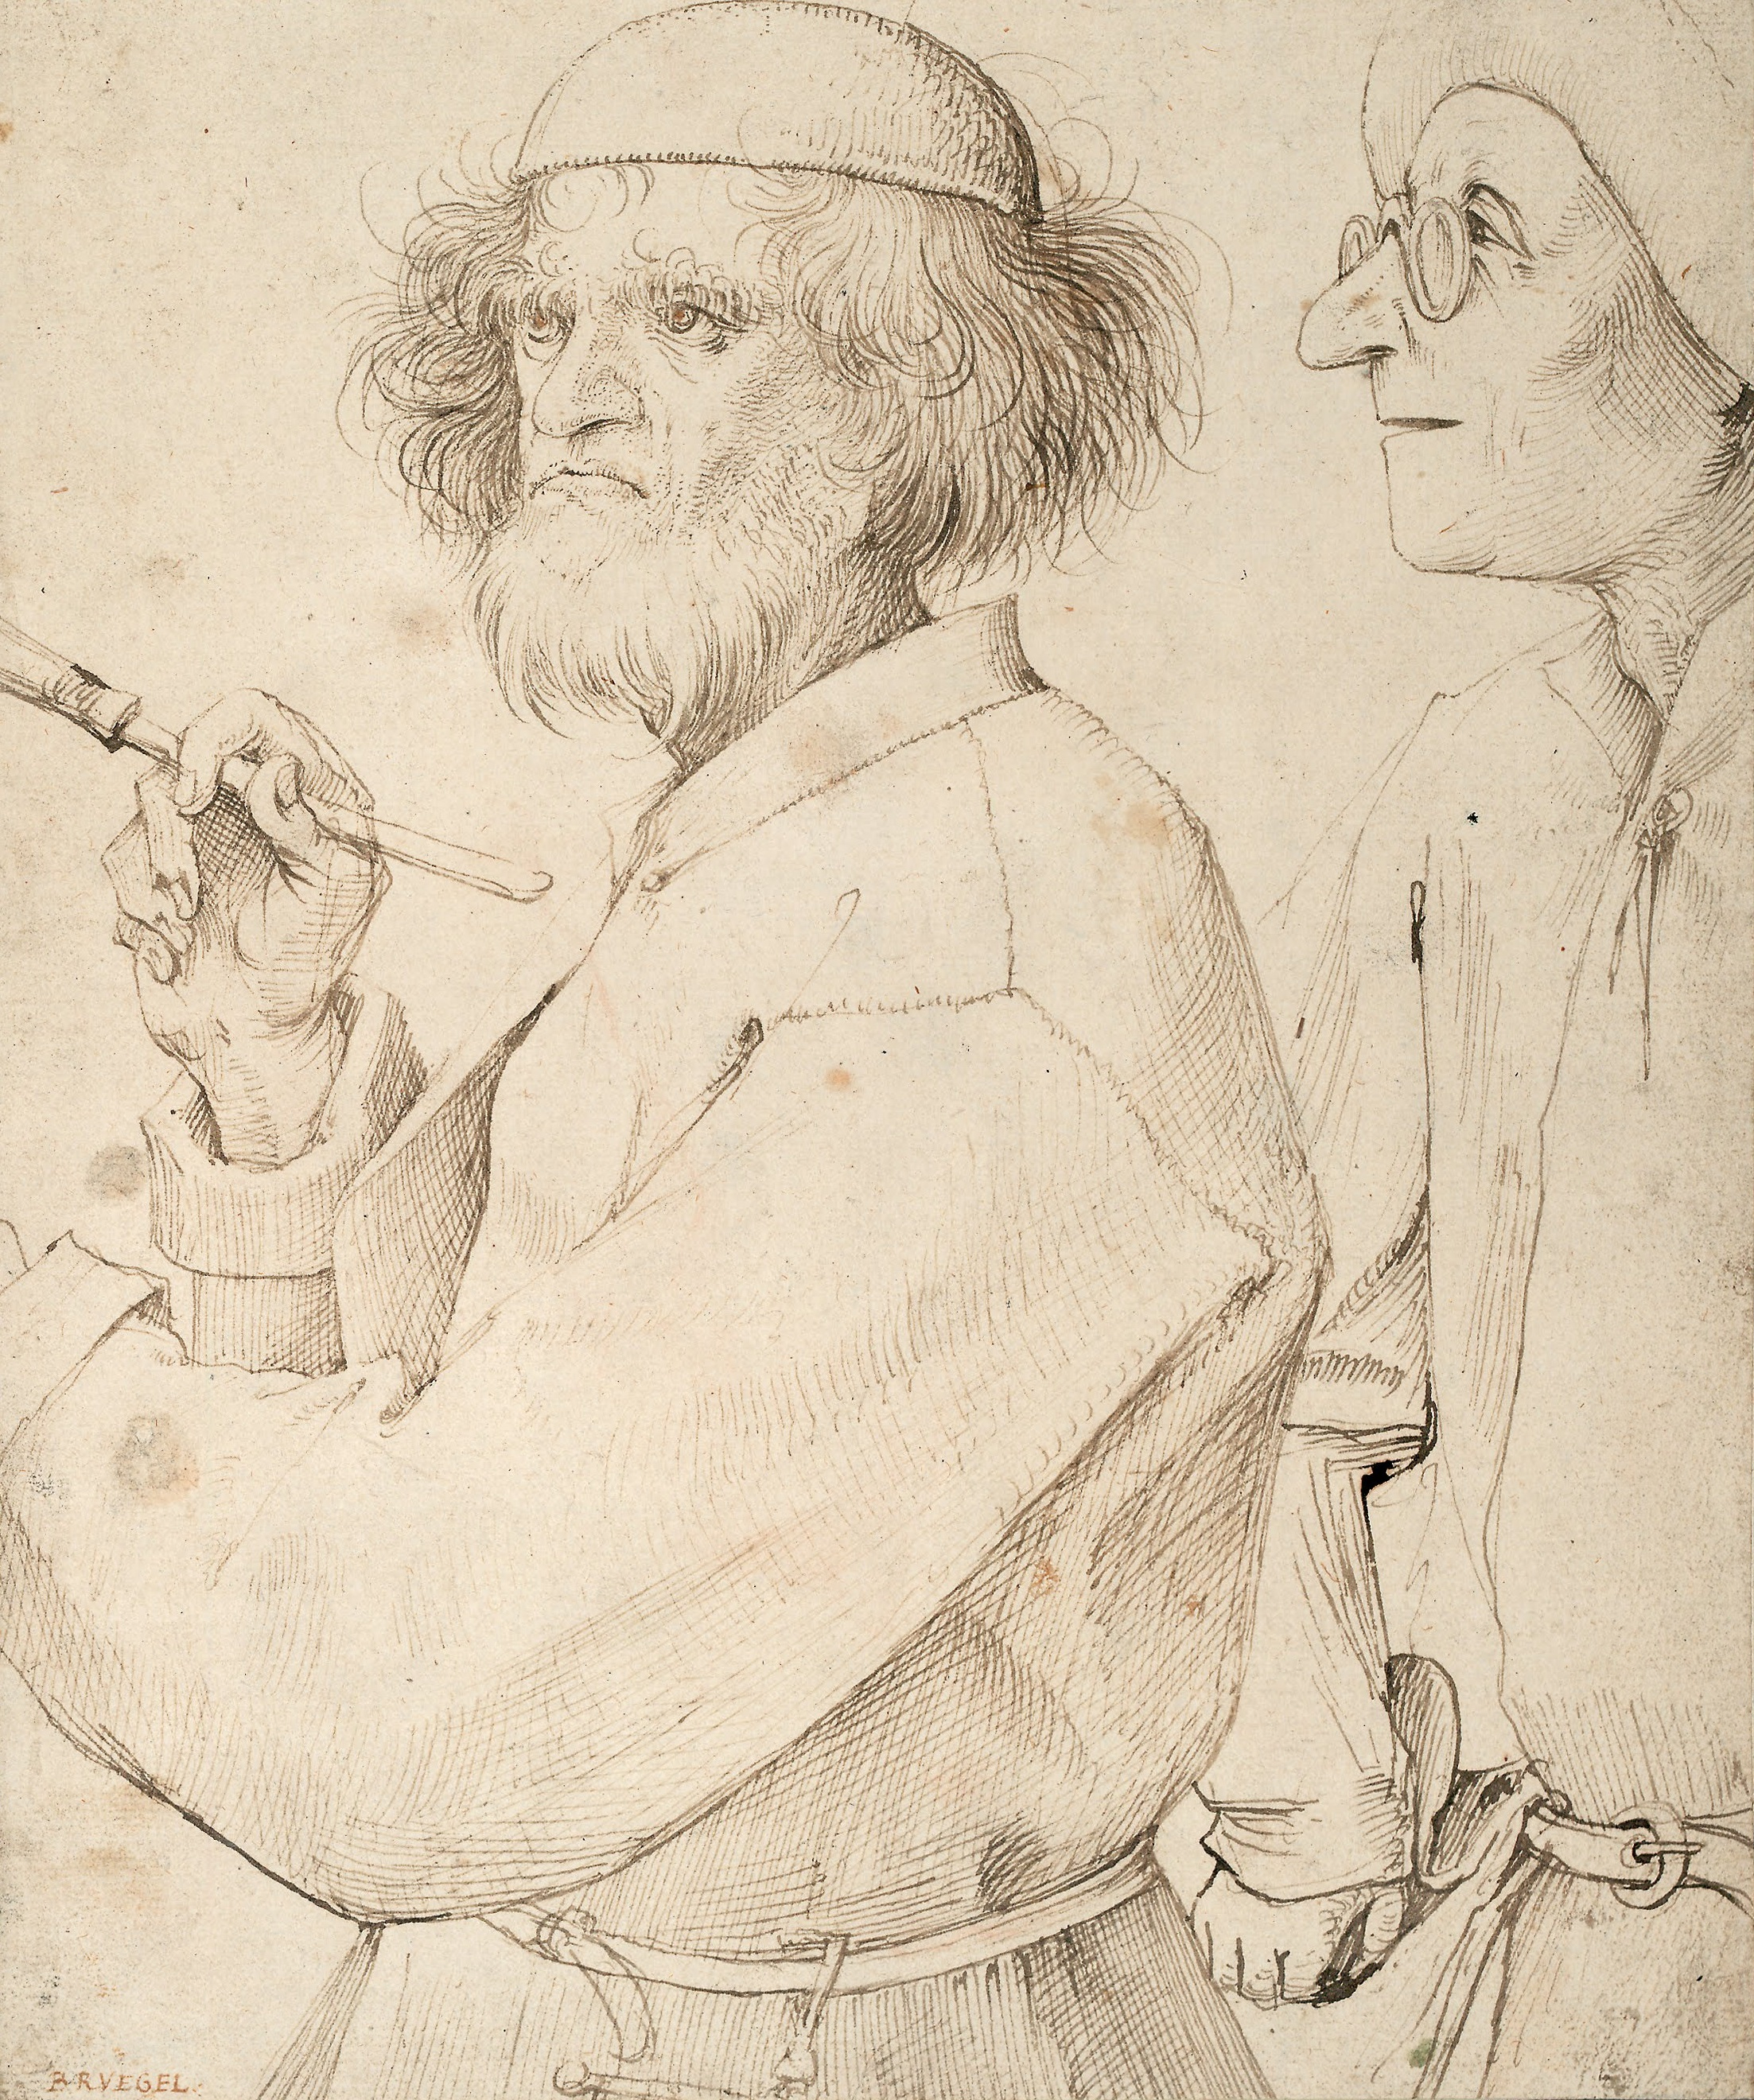
\includegraphics[height=0.3\textheight,keepaspectratio]
                          {images/brueghel.jpg}
  \caption{``O artista e o observador'' - Pieter Brueghel (ca. 1568)}
  \label{fig:1}
\end{figure}

Em seguida, encontra-se uma proposta bastante inovadora, sobretudo
para um tratado do séc. XVI: se houvesse ``fantasia e memória''
suficientemente boas e ``olhos invisíveis'', o retrato poderia ser
mais perfeito do que a própria realidade. Por fim, surge uma sugestão
completamente arrojada e muitos séculos à frente da época de F. d'H.,
a de que a presença dos rostos dos criados na sala pudesse
secretamente influenciar o retrato do e aparecer sobrepostos no rosto
do senhor.

No capítulo 11º, F. d'H. decide marcar, aqui sim, uma contribuição sua
como original, a de que a um espelho acrescenta à pintura ``um não sei
quê de mais graça e venustidade'', e que permite detectar erros. Alude
directamente a Leon Alberti, seu contemporâneo e, de certa forma,
concorrente\cite[p.41]{holanda}:

\begin{quote}
  [...] é mui acertado o que eu tenho descoberto há poucos anos do
  juízo do espelho, o qual creio que já dos antigos seria achado e
  mais segundo o louva Leo Baptista num livro que novamente se
  imprimiu em pintura. [...] Mas eu, sem ter nenhuma notícia do tal
  livro, tinha já escrito este.
\end{quote}

Por fim, é neste capítulo que Francisco d'Holanda abre uma rara
excepção à sua habitual predisposição para o auto-elogio, na forma de
mais uma relato em que intervem o seu pai. O imperador Carlos V teria
disto a António d'Holanda que preferia o seu retrato tirado por este
artista em iluminação, ao que dele fez o pintor Ticiano de
Veneza. Neste ponto F. d'H. rende-se à verdade ``Porém, eu dou
vantagem a Ticiano''\cite[p.42]{holanda}

\section{Conclusão}

No prólogo que abre ``Do Tirar Polo Natural'', o leitor depara-se com
uma densa lista de pormenores anedóticos de duvidosa relevância da
sobre a viagem que lhe origem ao diálogo. Com efeito, o peso das
referências autobiográficas nesta obra, tal em todas as outras do
autor, faz com que seja fácil ler os livros de F. d'H. como tratados
de auto-promoção gratuita de um autor com uma ideia desmesuradamente
grande de si próprio.\footnote{Talvez o expoente desta valorização
  seja a afirmação ``Francisco d'Holanda já nasceu
  pintor!''\cite{teresa-desenho}}. Esta dimensão está de facto
presente nos livros de F. f'H. e parece ser uma espécie de figura de
estilo da época.

No entanto, as referências autobiográficas não são de todo
inconsequentes: elas ocultam ocultam todo um enquadramento
sócio-político da obra e do próprio autor: como revela a análise de
José da Felicidade Alves, nas breves menções a nomes de povoações e de
personalidades, consolida-se a ideia de F. d'H. como homem
comprometido com diversas incumbências procedentes da corte do rei
D. João III. Em cada livro seu, sobretudo nos dois últimos dedicados
como ``lembranças'' a D. Sebastião, neto de D. João III,
F. d'H. esforça-se por sublinhar esta participação e proximidade, sem
esquecer de referir a herança e linhagem artística do seu pai, na
esperança que isso lhe seja recompensado na forma de novas
encomendas. Nesta perspectiva, toda a obra de Francisco da Holanda é
um \emph{curriculum vitae} rolante de recomendações profissionais.

Por outro lado, é no conteúdo filosófico-teórico inovador que a sua
obra realmente se destaca e brilha. Por exemplo, ainda que muitos dos
``preceitos'' sobre retrato que Francisco d'Holanda oferece neste
tratado sejam simples indicações de estilo maneirista sobre o
tratamento dos diferentes pormenores fisionómicos do retratado, há um
outro plano de leitura que trata da relevância da relação psicológica
invisível entre artista, modelo e a própria Arte. Há assim indícios de
uma proposta da obra pictórica como fonte de significado mais poderosa
do que a própria realidade. Os conceitos que surgem nesta obra da fase
inicial de F. d'H. viriam a desaguar, por exemplo, na ideia de
``desenho interno'', que precede por algumas décadas a proposta
equivalente de Zuccaro.\cite{holanda-desenho}.

Imbuído de uma admiração profunda pelos ícones do alto renascimento,
mas nascido já numa certa confusão pós-renascentista, F. d'H. parece
sobreestimar-se como artista e subestimar-se como filósofo. Deseja
tornar-se no humanista completo, no artista ideal da Renascença, mas
encontra em Portugal pouco eco às suas ambições.

\printbibliography[heading=bibliography,title={Bibliografia}]

\end{document}
